\documentclass[11pt,a4paper]{article}
\usepackage{fontspec}
\setmainfont{NotoSerifCJKkr-Regular.otf}[Path=fonts/,BoldFont=NotoSerifCJKkr-Bold.otf,ItalicFont=NotoSerifCJKkr-Regular.otf]
\setsansfont{NotoSerifCJKkr-Regular.otf}[Path=fonts/,BoldFont=NotoSerifCJKkr-Bold.otf]
\setmonofont{DejaVu Sans Mono}[Scale=0.79]
\XeTeXlinebreaklocale "ko"
\XeTeXlinebreakskip=0pt plus 1pt
\usepackage[margin=23mm,top=23mm,bottom=23mm,headheight=15pt]{geometry}
\usepackage{amsmath,amssymb,amsthm,mathtools}
\usepackage{booktabs,tabularx,longtable,array,graphicx,float}
\usepackage[dvipsnames]{xcolor}
\usepackage{enumitem,caption,fancyhdr,titlesec}
\usepackage{tikz}
\usetikzlibrary{arrows.meta,positioning,calc}
\usepackage{hyperref}
\providecommand{\tightlist}{\setlength{\itemsep}{0pt}\setlength{\parskip}{0pt}}
\newcommand{\passthrough}[1]{#1}
\hypersetup{unicode=true,colorlinks=true,linkcolor=MidnightBlue,urlcolor=MidnightBlue,citecolor=MidnightBlue,pdftitle={WU088 HH PHYS17: 상관된 결함의 매개변수 응답과 단조성},pdfauthor={WU088 HH 연구}}
\urlstyle{same}
\setlength{\emergencystretch}{3em}
\setlength{\parskip}{0.34em}
\setlength{\parindent}{1em}
\widowpenalty=10000\clubpenalty=10000
\linespread{1.10}
\setlist{itemsep=0.18em,topsep=0.35em,leftmargin=1.6em}
\captionsetup{font=small,labelfont=bf}
\renewcommand{\figurename}{그림}
\renewcommand{\tablename}{표}
\renewcommand{\contentsname}{목차}
\renewcommand{\refname}{참고 문헌과 원자료}
\renewcommand{\proofname}{증명}
\titleformat{\section}{\large\sffamily\bfseries\color{MidnightBlue}}{\thesection}{0.7em}{}
\titleformat{\subsection}{\sffamily\bfseries}{\thesubsection}{0.7em}{}
\pagestyle{fancy}\fancyhf{}
\fancyhead[L]{\small\sffamily WU088\_HH / PHYS17 이론}
\fancyhead[R]{\small\sffamily 2026-10-13 KST}
\fancyfoot[C]{\thepage}
\newcommand{\dd}{\mathrm d}
\newcommand{\diag}{\operatorname{diag}}
\newcommand{\ex}{\operatorname{exact64}}
\newcommand{\BB}{\mathcal B}
\newcommand{\HF}{\mathcal H_F}
\newcommand{\R}{\mathsf R}
\newcommand{\RF}{\mathsf R_F}
\newcommand{\ew}{e_w}
\newcommand{\exx}{e_x}
\newcommand{\nS}[1]{\left\lVert#1\right\rVert_S}
\newcommand{\nI}[1]{\left\lVert#1\right\rVert_\infty}
\newcommand{\magv}{\operatorname{mag}}
\newtheorem{theorem}{정리}
\newtheorem{lemma}{보조정리}
\newtheorem{proposition}{명제}
\theoremstyle{definition}\newtheorem{definition}{정의}

\newcommand{\ReviewDecision}{PROMOTE\_SCOPED}
\newcommand{\ReviewExplanation}{독립 과학 검토가 현재 전제 범위의 채택을 판정했다. 독립 유리수 산술 29개 항목, Wolfram+xAct 텐서 6개 항목과 scalar 15개 성분이 통과했으며, 남은 blocking finding은 없다.}

\begin{document}
\begin{center}
{\color{MidnightBlue}\sffamily\large WU088\_HH \quad PHYS17 이론 연구}\\[5mm]
{\LARGE\bfseries 상관된 endpoint 결함의 매개변수 응답}\\[3mm]
{\Large\bfseries C$^2$ source 구성, 공통 adjoint와 전역 단조성}\\[4mm]
{\large 2026년 10월 13일 KST}
\end{center}
\vspace{2mm}\noindent\rule{\textwidth}{0.6pt}
\section*{초록}
동일 초기 COMMON, 고정된 admissible 계수 선택 $\alpha$, 공유된 전역 매개변수 $(\lambda,b)\in[0,1]^2$에서 실제 두 half 경로와 Full 경로의 endpoint 차이 $d=g_2-g_F$ 및 온도 차이 $\Delta T=T_2-T_F$를 미분한다. PHYS16에서 얻은 유한 결함과 원 signed source gradient, Hessian, mixed derivative 및 PHYS09/11/14의 실제 carry를 재사용한다. 작은 결함 $d$를 먼저 인수로 추출하는 정확한 미분 잔차식을 구성하여, 각 경로의 독립 sensitivity 상자를 뺄 때 생기는 구간 폭을 줄인다.

새 source 구성은 $U=(F_w+\chi_HF_x)/(ne)$와 온도를 보존하는 방향 $\xi=e_x+(w/\Pi)e_w$로부터 helium 열원 계수 $k_{w\mathrm{He}}=(U-xDU[\xi])/f$ 및 그 도함수를 직접 회수한다. 이에 따라 exact density pullback의 1차 응답이 원 $C^2$ 자료에서 닫힌다. 동일 stage 증분의 도함수를 gas movement와 photon opacity에 공유하고, 비가환 수송을 유지한 일곱 photon sector를 미분한다. 원 Full 전처리 $C,B,q,S$와 하나의 온도 covector가 모든 forcing과 feedback을 같은 endpoint에서 전달한다.

실제 외향 구간 계산은
\[
\partial_\lambda\Delta T\in[-1.009599125635,-0.8137506081166]\times10^{-8}\ \mathrm K,
\]
\[
\partial_b\Delta T\in[6.776348385589,7.185335549648]\times10^{-5}\ \mathrm K
\]
를 준다. 따라서 이 계열에서 $\Delta T$는 $\lambda$에 대해 감소하고 $b$에 대해 증가한다. $\lambda$의 직접 forcing과 state feedback은 모두 음수이며, $b$의 양의 직접 forcing은 작은 음의 feedback을 포함한 뒤에도 양수다. 기존 $\Delta T<0$ 포함과 결합하면, 두 half의 낮은 온도는 유지되면서 birth가 그 차이를 줄이는 구조를 얻는다.

Wolfram Language에서 공식 xAct/xTensor를 실제 실행하여 텐서 항등식 6개와 scalarㆍ행렬 성분 항등식 15개를 정확히 검산한다. 독립 Fraction 검토, 원전 대응, 원 입력의 identity, 실행 기록 및 다음 mixed-response 계약을 함께 제시한다.\cite{Neumaier1989Sensitivity,Rump1990Sensitivity,MargossianBetancourt2022Implicit,phys16,app17}

\noindent\fcolorbox{MidnightBlue!45}{MidnightBlue!3}{%
\parbox{\dimexpr\textwidth-2\fboxsep-2\fboxrule\relax}{%
\textbf{연구 판정}\quad \ReviewDecision\par
\small \ReviewExplanation}}
\newpage
\begingroup\small\setlength{\parskip}{0pt}\tableofcontents\endgroup
\vspace{4mm}
\noindent\textbf{읽기 순서.} 제1절은 새 수치 결과와 물리적 귀결을 제시한다. 이어지는 정리들은 원 잔차에서 응답식, source closure, photon 미분, inverse와 adjoint 전달을 실제로 유도한다. 후반부는 직접 forcingㆍfeedback, 검산ㆍ문헌, 다음 연구 의무와 재현 경로를 설명한다.
\newpage
\section{새 연구 결과와 물리적 귀결}
\label{sec:results}
현재 연구 단위는 PHYS16에서 열린 \texttt{HH\_DEFECT\_PARAMETER\_RESPONSE}를 수행한다. $\lambda$는 원 HH source의 세기, $b$는 같은 birth packet의 세기다. 두 매개변수는 각 단계마다 같은 값을 갖는다. 열에너지 좌표는 $w\,[\mathrm{eV/H}]$, $f_2$는 endpoint에서 보존된 정확한 $n_{\rm He}/n_{\rm H}$ 비이며,
\[
g=(x_{\rm HII},y_{\rm HeII},y_{\rm HeIII},w)^T,\qquad
d=g_2-g_F,\qquad d_e=(1,f_2,2f_2,0)d
\]
로 정의한다. 원 $\alpha$를 고정한 채 $\lambda$ 또는 $b$만 미분한다. 시간은 $h=625000000\,\mathrm s$, $t_0=160000000000\,\mathrm s$, 두 half의 최종 시각은 $t_2=161250000000\,\mathrm s$다.

\begin{table}[htbp]\centering\scriptsize
\caption{같은 전역 매개변수에 대한 실제 endpoint 결함의 1차 응답. 두 열은 각각 단위 무차원 매개변수당 값이다.}\label{tab:responses}
\setlength{\tabcolsep}{3pt}\begin{tabular}{lll}\toprule
관측량 & $\partial_\lambda$ 포함 & $\partial_b$ 포함\\\midrule
수소 이온화 차이 $d_{x,\theta}$ & $[1.366697436231,1.689925910794]\times10^{-13}$ & $[-3.127854741570,-2.993844665600]\times10^{-9}$\\
He II 차이 $d_{y,\theta}$ & $[5.928617637399,9.956711152243]\times10^{-17}$ & $[1.608398971389,2.774242695334]\times10^{-15}$\\
He III 차이 $d_{z,\theta}$ & $[4.796181447457,6.313426646227]\times10^{-18}$ & $[4.434566279600,4.807180040710]\times10^{-16}$\\
열에너지 차이 [eV/H] $d_{w,\theta}$ & $[-1.686607512876,-1.370408263621]\times10^{-12}$ & $[-3.253014902391,-3.107335579349]\times10^{-10}$\\
전자 수 차이 [H당] $d_{e,\theta}$ & $[1.366754605418,1.690019031785]\times10^{-13}$ & $[-3.127854534459,-2.993844355539]\times10^{-9}$\\
온도 차이 [K] $\Delta T_\theta$ & $[-1.009599125635,-0.8137506081166]\times10^{-8}$ & $[6.776348385589,7.185335549648]\times10^{-5}$\\
\bottomrule\end{tabular}\end{table}


표의 구간은 \texttt{run02}의 실제 외측 결과이며, 매개변수 직사각형 전체를 포함한다. 두 gas 좌표의 경우 상관식을 사용한 구간 폭의 개선은 $\lambda$의 $d_x$에서 약 $1.04\times10^4$배, $d_w$에서 약 $1.44\times10^4$배다. $b$의 해당 두 좌표에서는 각각 약 $42.5$배와 $41.3$배다. 비교 대상은 동일한 이전 $g_{2,\theta}$와 $g_{F,\theta}$ 포함을 독립적으로 뺀 상자다. 이 수치는 새 sample이나 fitting 대신 기존 입력 사이의 정확한 관계를 유지한 효과를 나타낸다.\cite{app17}

\subsection{두 매개변수의 작용}
$\partial_\lambda d_x>0$, $\partial_\lambda d_w<0$이므로 HH 세기를 높이면 두 half와 Full 사이의 추가 이온화 차이가 커지고 열에너지 차이는 더 음수가 된다. 유한 온도 분모의 변화까지 포함한 $\partial_\lambda\Delta T$도 음수다. 반면 $\partial_bd_x<0$, $\partial_bd_w<0$인데도 $\partial_b\Delta T>0$이다. 온도 응답의 정확한 식에서 입자 수 차이에 곱해지는 항이 함께 작용하기 때문이다. 에너지 성분만의 부호로 온도 응답을 대신하지 않고, 뒤의 공통 covector가 두 효과를 같은 분모에서 결합한다.

PHYS16의 $\Delta T\in[-1.585967387181453,-1.210819969055199]\times10^{-3}\,\mathrm K$는 현재 입력으로 재사용된다. 따라서 $b$를 키우면 이 음의 결함을 줄이고, $\lambda$를 키우면 조금 더 크게 만든다. 각 축의 단위 변화에 대한 전역 적분 포함은 그림~\ref{fig:finite}에 보였다. 같은 고정 $\alpha$와 같은 다른 매개변수에서 기준점으로부터의 변화를 나타내는 외측 영역이다.\cite{phys16,app17}

\begin{figure}[htbp]
\centering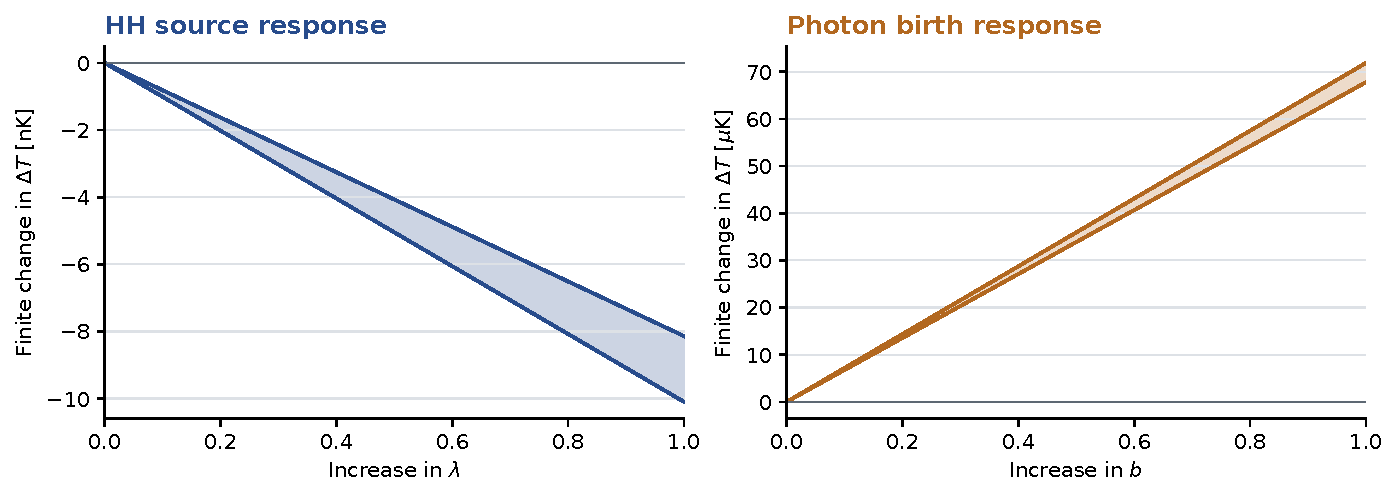
\includegraphics[width=\textwidth]{finite_parameter_envelopes.pdf}
\caption{실제 1차 응답 포함을 적분한 유한 변화 영역. 왼쪽은 $\lambda$ 변화에 따른 감소를 nK 단위로, 오른쪽은 $b$ 변화에 따른 증가를 $\mu$K 단위로 나타낸다. 채색 영역은 모든 동일 계열의 변화에 대한 외측 포함이다. 아래쪽 좌표의 0은 각 비교의 동일 계열 기준점이다.}
\label{fig:finite}
\end{figure}

\hypertarget{uxb300uxc0c1-uxc804uxc81cuxc640-uxd45cuxae30}{%
\section{대상, 전제와 표기}\label{uxb300uxc0c1-uxc804uxc81cuxc640-uxd45cuxae30}}

같은 초기 COMMON과 하나의 admissible 고정 계수 선택 \(\alpha\)에 대해 두 전역 매개변수 \(\theta=(\lambda,b)\in[0,1]^2\)를 Full과 실제 두 half 경로에 공유한다. 미분할 매개변수는 \(\theta\in\{\lambda,b\}\) 하나이며 점은 도트로도 표기한다. 시간, 밀도, 원 상수, 수송 사상, COMMON의 미래 매개변수 도함수는 고정한다. 원 source family의 작은 열린 매개변수 확장 덕분에 닫힌 rectangle의 경계에서도 해당 1차 미분을 정의한다.

기체 좌표와 endpoint는

\[
g=(x,y,z,w)^T,\quad y_*=g_2,\quad d=g_2-g_F,\quad
v=g_{1,\theta},\quad u=g_{2,\theta},\quad s=g_2-g_1
\]

로 둔다. 이하 \(y_*\)는 두 번째 endpoint 벡터이고, \(y\)는 He II fraction이다. \(w\)의 단위는 eV/H이며 \(\lambda,b\)는 무차원이다. \(h=625000000\ \mathrm{s}\), Full 길이는 \(2h\)이다. 동일 endpoint 시각의 정확한 density ratio를 \(f=f_2=\operatorname{exact}(n_{\mathrm{He},2}^{\mathrm{stored}})/\operatorname{exact}(n_2)\)라 둔다. 물리상수 \(c,k_B\) 및 eV-to-erg leaf를 원 값으로 유지한다.

사용하는 가정은 다음과 같다.

\begin{enumerate}
\def\labelenumi{\arabic{enumi}.}
\tightlist
\item
  원 4차원 convex \(X\)의 내부 hull에 \(g_1,g_2,g_F\)와 필요한 선분·density pullback이 포함된다. source와 실제 implicit root family는 상속된 \(C^2\) family이다.
\item
  같은 고정 \(C,B,S,q\)가 \(X\)에서 \(\lvert I-CH_g(g;\lambda,b)\rvert\le B\), \(\lVert S^{-1}BS\rVert_\infty\le q<1\)을 만족한다. \(H=H_F\)는 Full 잔차다.
\item
  PHYS09/11/14의 원 1차 gas·photon carry와 PHYS16의 상관된 \(d,s\), 잔차 포함을 재사용한다. 원 signed gradient/Hessian은 부호 clipping을 하지 않는다.
\item
  현재 nonphoto source는 원 FT03의 CI·RR·DR graph이다. HI threshold \(\chi_H\)는 실제 source의 동일 captured leaf이다. 추가 source 성분은 별도 \(B\) 항으로 명시한다.
\end{enumerate}

이 가정과 원본 identity는 PHYS16의 \nolinkurl{contracts/PARAMETER_RESPONSE_CONTRACT.json}, PHYS15의 \nolinkurl{theory/ASSUMPTIONS_AND_BINDINGS_KO.md} 및 PHYS16의 \nolinkurl{evidence/intake/SOURCE_COOLING_AUDIT_KO.md}에 연결된다. 다음 유도에서 정칙성은 \(C^2\) 안에 유지된다.

원 source 포함의 적용 위치는 아래와 같다. 새로운 연결식이 원 \(X\) 밖의 source 값을 요구하지 않는다.

\begin{longtable}[]{@{}
  >{\raggedright\arraybackslash}p{(\columnwidth - 2\tabcolsep) * \real{0.5000}}
  >{\raggedright\arraybackslash}p{(\columnwidth - 2\tabcolsep) * \real{0.5000}}@{}}
\toprule\noalign{}
\begin{minipage}[b]{\linewidth}\raggedright
식의 평가점
\end{minipage} & \begin{minipage}[b]{\linewidth}\raggedright
도함수 입력과 포함 근거
\end{minipage} \\
\midrule\noalign{}
\endhead
\bottomrule\noalign{}
\endlastfoot
\(g_1,g_2\) 및 \(g_1+ts\) & 원 first-half/실제 second-half root hull의 convex hull \(\subset X\); Full nonphoto/q box Hessian과 centre-to-hull gradient 포함 \\
\(g_1\)의 온도 정렬점 \(g_*=\Psi(g_1)\)와 \(g_1+t(g_*-g_1)\) & PHYS15에서 exact density ratio와 내부 hull로 검토한 pullback; PHYS16 적용에서 같은 값을 재사용 \\
\(g_2-td,\ 0\le t\le1\) & PHYS16에서 포함한 실제 \(d=g_2-g_F\)와 원 \(g_2,g_F\)의 공통 convex \(X\) \\
P2의 \(H_{gg}\)와 \(H_{g\theta}\) & 원 Full \texttt{SOURCE\_BOX.json}의 잔차 gas Hessian 및 mixed gas/parameter Hessian; \(\lambda\) slot 4, b slot 5 \\
\end{longtable}

centre 자료를 이용해 값·gradient 포함을 좁힐 때도 Hessian의 권위 영역은 원 \(X\)이다. Whole-X Hessian을 새 centred Hessian 값으로 바꾸거나 추가 smoothness를 가정하지 않는다.

\hypertarget{uxc815uxb9ac-1-uxc791uxc740-endpoint-uxcc28uxc774uxb97c-uxba3cuxc800-uxc778uxc218-uxbd84uxd574uxd55c-uxbbf8uxbd84uxc2dd}{%
\section{정리 1 --- 작은 endpoint 차이를 먼저 인수 분해한 미분식}\label{uxc815uxb9ac-1-uxc791uxc740-endpoint-uxcc28uxc774uxb97c-uxba3cuxc800-uxc778uxc218-uxbd84uxd574uxd55c-uxbbf8uxbd84uxc2dd}}

\[
H(g)=g-g_0-2hB_2(g,\lambda)-VL_F(g)Q_F(b),\quad
H(g_F)=0,\quad r=H(g_2).
\]

\[
J_y=H_g(g_2),\qquad J_F=H_g(g_F),
\]

\[
\mathcal L(d)v_0=\int_0^1H_{gg}(g_2-td)[d,v_0]dt,\qquad
\mathcal G_\theta=\int_0^1H_{g\theta}(g_2-td)dt
\]

라 두면 정확히

\[
J_y-J_F=\mathcal L(d),\quad
H_\theta(g_2)-H_\theta(g_F)=\mathcal G_\theta d,
\]

\[
\boxed{J_Fd_\theta=f_\theta,
\qquad f_\theta=r_\theta-\mathcal L(d)u-\mathcal G_\theta d.}
\tag{1}
\]

\textbf{증명.} \(H(g_F;\theta)=0\)을 미분하면 \(J_F(g_{2,\theta}-d_\theta)+H_\theta(g_F)=0\)이다. 한편 \(r_\theta=J_yu+H_\theta(g_2)\)다. 두 식을 빼고 \(H_g\)와 \(H_\theta\)에 각각 선분 적분을 적용하면 (1)이 성립한다. \(H_{gg},H_{g\theta}\)의 연속성만 사용한다. \(\square\)

따라서 새 forcing \(f_\theta\)의 모든 feedback 항은 작은 \(d\)를 명시적으로 인수로 갖는다. 이와 동치인 endpoint 기준식은

\[
\boxed{J_yd_\theta=f_\theta+\mathcal L(d)d_\theta.}
\tag{2}
\]

원 Full 기체 1차 carry \(g_{F,\theta}\)를 사용할 때에는

\[
J_yd_\theta=r_\theta-\mathcal L(d)g_{F,\theta}-\mathcal G_\theta d
\tag{3}
\]

도 같은 \(d_\theta\)를 포함한다. 식 (3)은 두 경로의 원 1차 carry와 상관 잔차의 독립 연결로 사용할 수 있다.

\hypertarget{uxc2e4uxc81c-source-slotuxacfcuxc758-uxb300uxc751}{%
\subsection{실제 source slot과의 대응}\label{uxc2e4uxc81c-source-slotuxacfcuxc758-uxb300uxc751}}

현재 \(H\)의 명시적 매개변수 미분은

\[
H_\lambda=-2h q_2\nu_H,\qquad
H_{g\lambda}=-2h\nu_H\otimes Dq_2,
\]

\[
H_b=-2VL_FJ_\gamma,\qquad
H_{gb}=2\sum_j\frac{\ell_jJ_{\gamma j}}{D_{Fj}^2}\nu_j e_x^T,
\quad\ell_j=2ha_{2j}.
\tag{4}
\]

여기서 \(\nu_H=(1,0,0,-\chi_H)^T\), \(J_\gamma=M_\gamma e_{24}\), \(D_{Fj}=1+\ell_j(1-x)\)이다. source export의 \texttt{G\_g\_lambda{[}i{]}{[}j{]}}, \texttt{G\_g\_b{[}i{]}{[}j{]}}는 각각 residual{[}i{]}.hessian{[}j{]}{[}4{]}, residual{[}i{]}.hessian{[}j{]}{[}5{]}에 대응한다. \texttt{G\_gg}는 이미 Full \textbf{잔차} Hessian이다.

\hypertarget{uxc815uxb9ac-2-stage-movementuxc758-uxb3c4uxd568uxc218uxb97c-uxacf5uxc720uxd558uxb294-gas-uxc794uxcc28}{%
\section{정리 2 --- stage movement의 도함수를 공유하는 gas 잔차}\label{uxc815uxb9ac-2-stage-movementuxc758-uxb3c4uxd568uxc218uxb97c-uxacf5uxc720uxd558uxb294-gas-uxc794uxcc28}}

비광자 source를

\[
B_k(g,\lambda)=F_k(g)+\lambda q_k(g)\nu_H-2H_kw e_w
\]

로 쓴다. \(F_k\)는 원 nonphoto export이다. PHYS15/16에서

\[
s=hB_2(g_2)+VP_2,\qquad
r_g=h\{B_1(g_1)-B_2(g_2)\}
\]

를 얻었다. 같은 매개변수로 미분하면

\[
\boxed{s_\theta=h\{B_{2,g}(g_2)u+\delta_{\theta\lambda}q_2(g_2)\nu_H\}+VP_{2,\theta}.}
\tag{5}
\]

이 \(s_\theta\)는 정확히 \(u-v\)와 같으므로 보존된 두 sensitivity 포함과 교차할 수 있다. \(g_t=g_1+ts\), \(\delta B_t(g)=B_1(g)-B_2(g)\), \(\delta q_t=q_1-q_2\)로 두면

\[
\boxed{\begin{aligned}
r_{g,\theta}={}&h\{D\delta B_t(g_1)[v]+\delta_{\theta\lambda}\delta q_t(g_1)\nu_H\}\\
&-hB_{2,g}(g_2)s_\theta
-h\int_0^1B_{2,gg}(g_t)[s,v]dt
-h\delta_{\theta\lambda}\int_0^1Dq_2(g_t)[s]dt\,\nu_H.
\end{aligned}}
\tag{6}
\]

\textbf{증명.} 정확한 직접 미분은

\[
r_{g,\theta}=h\{B_{1,g}(g_1)v-B_{2,g}(g_2)u
+\delta_{\theta\lambda}[q_1(g_1)-q_2(g_2)]\nu_H\}.
\]

\(u=v+s_\theta\)를 넣는다. \(B_{1,g}(g_1)-B_{2,g}(g_2)\)는 \(D\delta B_t(g_1)-\int_0^1B_{2,gg}(g_t)[s,\cdot]\,dt\)이고, \(q_1(g_1)-q_2(g_2)=\delta q_t(g_1)-\int_0^1Dq_2(g_t)[s]\,dt\)다. 대입하면 (6)이 따른다. \(\square\)

식 (6)은 평균 source Jacobian 자체를 매개변수 미분한 표현을 endpoint \(B_{2,g}(g_2)s_\theta\)와 작은 \(s\)의 Hessian contraction으로 재구성한다. 원 \(H_1=H_2\)이므로 \(\delta B_t\)의 팽창항은 정확히 소거되고, \(B_{2,g}\)에는 \(-2H_2e_we_w^T\)를 유지한다.

\hypertarget{uxc815uxb9ac-3-cuxb2-nonphoto-jetuxc5d0uxc11c-he-thermal-derivativeuxb97c-uxc9c1uxc811-uxd68cuxc218}{%
\section{정리 3 --- \texorpdfstring{\(C^2\)}{C2} nonphoto Jet에서 He thermal derivative를 직접 회수}\label{uxc815uxb9ac-3-cuxb2-nonphoto-jetuxc5d0uxc11c-he-thermal-derivativeuxb97c-uxc9c1uxc811-uxd68cuxc218}}

이 정리는 density pullback의 작은 He 보정에 필요한 도함수를 닫는다. \(f,n\)은 endpoint 2의 고정 값이고

\[
e=x+f(y+2z),\quad \Pi=1+f+e,\quad T=C_Tw/\Pi,\quad
\ell_e=(1,f,2f,0)
\]

이다. 다음 정규화된 화학·열 조합과 온도를 유지하는 \(x\) 방향을 정의한다.

\[
U(g)=\frac{F_w(g)+\chi_HF_x(g)}{ne},\qquad
\xi(g)=e_x+\frac{w}{\Pi}e_w.
\tag{7}
\]

원 source에서

\[
F_x=ne\{(1-x)\beta_H-x\alpha_H\},
\]

\[
F_w=ne\{-\chi_H(1-x)\beta_H-x\kappa_H
+f k_{w\mathrm{He}}(y,z,T)\}.
\]

따라서

\[
U(g)=-x\{\kappa_H(T)+\chi_H\alpha_H(T)\}
+f k_{w\mathrm{He}}(y,z,T).
\tag{8}
\]

\(DT[\xi]=0\)이고 \(Dy[\xi]=Dz[\xi]=0\)이므로 식 (8)의 고정 온도 \(x\) 미분을 취하면

\[
DU[\xi]=-[\kappa_H(T)+\chi_H\alpha_H(T)].
\]

그러므로

\[
\boxed{k_{w\mathrm{He}}(g)=\frac{U(g)-xDU(g)[\xi(g)]}{f}.}
\tag{9}
\]

임의의 기체 방향 \(v_0\)에 대해 이를 한 번 미분하면

\[
\boxed{\begin{aligned}
Dk_{w\mathrm{He}}(g)[v_0]
=\frac{1}{f}\bigg\{
DU[v_0]-v_{0x}DU[\xi]
-x\big[D^2U[v_0,\xi]+DU[D\xi[v_0]]\big]\bigg\},\\
D\xi[v_0]=\left[\frac{v_{0w}}{\Pi}
-\frac{w\ell_ev_0}{\Pi^2}\right]e_w.
\end{aligned}}
\tag{10}
\]

\textbf{증명.} (8)은 원 hydrogen CI 항을 동일 \(\chi_H\)로 소거한 source 항등식이다. \(\xi\)를 따라 온도와 He fractions가 고정되므로 첫 방향 미분에서 수소 항의 계수만 남는다. (9)에 ordinary product·chain rule을 적용하고 \(\xi\)의 도함수를 계산하면 (10)을 얻는다. (9)는 현재 \(g\)에서의 국소 값·도함수 항등식으로, \(x=0\)까지 source를 평가할 필요가 없다. \(\square\)

\hypertarget{uxc800uxc7a5uxb41c-source-jetuxc5d0-uxbc14uxb85c-uxc801uxc6a9uxd558uxb294-uxacc4uxc0b0uxc2dd}{%
\subsection{저장된 source Jet에 바로 적용하는 계산식}\label{uxc800uxc7a5uxb41c-source-jetuxc5d0-uxbc14uxb85c-uxc801uxc6a9uxd558uxb294-uxacc4uxc0b0uxc2dd}}

\(L=F_w+\chi_HF_x\)라 두면 \(e\)의 Hessian은 0이므로

\[
DU[v_0]=\frac1n\left(\frac{DL[v_0]}e-
\frac{L\ell_ev_0}{e^2}\right),
\]

\[
\boxed{D^2U[v_0,z_0]=\frac1n\left\{
\frac{D^2L[v_0,z_0]}e
-\frac{DL[v_0]\ell_ez_0+DL[z_0]\ell_ev_0}{e^2}
+\frac{2L(\ell_ev_0)(\ell_ez_0)}{e^3}
\right\}.}
\tag{11}
\]

식 (9)--(11)의 입력은 Full \texttt{nonphoto{[}0{]}}, \texttt{nonphoto{[}3{]}}의 value, gas gradient, signed gas Hessian뿐이다. \(e,f,\Pi\)가 양수인 원 hull에서 모두 정칙하다. PHYS16의 cooling-cone 값 포함과 식 (9)의 값 포함은 같은 함수에 대한 두 포함으로 교차할 수 있다. 도함수 포함은 식 (10)--(11)에서 직접 얻는다.

\hypertarget{uxc815uxb9ac-4-exact-density-pullbackuxc758-uxc0c1uxad00uxb41c-1uxcc28-closure}{%
\section{정리 4 --- exact density pullback의 상관된 1차 closure}\label{uxc815uxb9ac-4-exact-density-pullbackuxc758-uxc0c1uxad00uxb41c-1uxcc28-closure}}

\[
\sigma=y+2z,\quad e_k=x+f_k\sigma,\quad
\Pi_k=1+f_k+e_k,\quad \Delta f=f_1-f_2,\quad r_n=n_1/n_2,
\]

\[
r_e=r_ne_1/e_2,
\quad\delta w=-w\Delta f(1+\sigma)/\Pi_1,
\quad g_*=g+\delta w e_w.
\]

그러면 \(T_2(g_*)=T_1(g)\)이고

\[
F_1(g)=r_eF_2(g_*)+n_1e_1\Delta f\,k_{w\mathrm{He}}(g_*)e_w,
\quad q_1(g)=r_nq_2(g_*).
\tag{12}
\]

작은 차이를 보존하는 값은

\[
r_e-1=(r_n-1)+r_n\Delta f\,\sigma/e_2.
\]

방향 \(v_0\)를 따라 \(\dot\sigma=v_{0y}+2v_{0z}\), \(\dot e_k=\ell_{e,k}v_0\)라 두면

\[
\boxed{Dr_e[v_0]=r_n\Delta f
\frac{e_2\dot\sigma-\sigma\dot e_2}{e_2^2},}
\tag{13}
\]

\[
\boxed{D\delta w[v_0]=-
\Delta f\left[
\frac{(1+\sigma)v_{0w}+w\dot\sigma}{\Pi_1}
-\frac{w(1+\sigma)\dot e_1}{\Pi_1^2}
\right].}
\tag{14}
\]

\(F=F_2\), \(q=q_2\), \(\delta F=F_1-F_2\), \(\delta q=q_1-q_2\), \(v_*=v_0+D\delta w[v_0]e_w\)로 줄여 쓰자. 정확히

\[
\boxed{\begin{aligned}
D\delta F(g)[v_0]={}&(r_e-1)DF(g)[v_0]+Dr_e[v_0]F(g_*)\\
&+r_e\delta w\int_0^1D^2F(g+t\delta w e_w)[e_w,v_0]dt\\
&+r_e(\partial_wF)(g_*)D\delta w[v_0]\\
&+n_1\Delta f\left\{
\dot e_1 k_{w\mathrm{He}}(g_*)
+e_1Dk_{w\mathrm{He}}(g_*)[v_*]
\right\}e_w,
\end{aligned}}
\tag{15}
\]

\[
\boxed{\begin{aligned}
D\delta q(g)[v_0]={}&(r_n-1)Dq(g)[v_0]\\
&+r_n\delta w\int_0^1D^2q(g+t\delta w e_w)[e_w,v_0]dt\\
&+r_n(\partial_wq)(g_*)D\delta w[v_0].
\end{aligned}}
\tag{16}
\]

여기서 \(\partial_wF\)와 \(\partial_wq\)는 \(w\) 좌표의 도함수다. 구현에서는 각각 \texttt{DF{[}:,3{]}}, \texttt{Dq{[}3{]}}로 명시한다.

\textbf{증명.} (12)를 \(v_0\)로 미분하고 \(Dg_*v_0=v_*\)를 사용한다. \(r_eDF(g_*)[v_0]-DF(g)[v_0]\)를 \((r_e-1)DF(g)[v_0]+r_e(DF(g_*)-DF(g))[v_0]\)로 나눈 뒤 마지막 차이에 Hessian 선분 적분을 적용한다. HH 식도 \(r_n\)이 고정인 같은 계산으로 따른다. He correction의 도함수는 (10)을 직접 대입한다. \(\square\)

식 (6)의 source-time 항은

\[
D\delta B_t(g)[v_0]=D\delta F(g)[v_0]+\lambda D\delta q(g)[v_0]\nu_H
\]

로 닫힌다. 현재 exact \(\Delta f\)는 약 \(-6.94525\times10^{-18}\)이고 이 작은 factor가 모든 density-normalization derivative 항에 유지된다. \(\Delta f=0\)이면 \(g_*=g\), \(D\delta w=Dr_e=0\)이므로 (15)--(16)은 정확히 \((r_n-1)DF[v_0]\), \((r_n-1)Dq[v_0]\)로 환원된다.

\hypertarget{uxc815uxb9ac-5-uxc6d0-photon-uxc77cuxacf1-sectoruxc758-1uxcc28-uxbbf8uxbd84}{%
\section{정리 5 --- 원 photon 일곱 sector의 1차 미분}\label{uxc815uxb9ac-5-uxc6d0-photon-uxc77cuxacf1-sectoruxc758-1uxcc28-uxbbf8uxbd84}}

\(R,R_F\)와 \(Z_0\)는 고정이고 \(J_\gamma=M_\gamma e_{24}\)이다. \(g_2\)에서

\[
\tau_j=ha_{2j}(1-x_2),\quad A=(I+\tau)^{-1},\quad
L=I-A,\quad A_F=(I+2\tau)^{-1},\quad L_F=I-A_F,
\]

\[
C_1=\tau A^2A_F,\quad C_2=\tau^2A^2A_F,\quad
Q_1=RZ_0+bJ_\gamma,\quad\Delta R=R^2-R_F.
\]

대각 연산자끼리의 곱은 성분별이다. 기체 전처리 \(C\)와 photon \(C_1,C_2\)는 구분한다. \(\delta_b=\delta_{\theta b}\)라 두면

\[
\dot Q_1=\delta_bJ_\gamma,\quad
\dot\tau_j=-ha_{2j}u_x,\quad
\dot A=-A^2\dot\tau,\quad \dot L=-\dot A,
\]

\[
\dot A_F=-2A_F^2\dot\tau,\quad \dot L_F=-\dot A_F,
\]

\[
\dot C_1=A^2A_F(1-2\tau A-2\tau A_F)\dot\tau,
\]

\[
\dot C_2=2\tau A^2A_F(1-\tau A-\tau A_F)\dot\tau.
\tag{17}
\]

첫 opacity 차이는 작은 scalar \(\zeta\)를 먼저 유지한다.

\[
\zeta_j=h\{c\sigma_j(n_2-n_1)(1-x_2)-a_{1j}s_x\},
\quad\Delta A_1=\zeta A_1A,
\]

\[
\dot\zeta_j=-h\{c\sigma_j(n_2-n_1)u_x+a_{1j}s_{\theta,x}\},
\quad \dot A_{1j}=ha_{1j}A_{1j}^2v_x,
\]

\[
\boxed{\dot{\Delta A}_1=\dot\zeta A_1A
+\zeta(\dot A_1A+A_1\dot A).}
\tag{18}
\]

\(K=I-LR\)라 두면 PHYS15의 각 \(p\) sector와 그 도함수는 다음과 같다.

\[
p_{op}=-K\Delta A_1Q_1,
\quad
\boxed{\dot p_{op}=\dot LR\Delta A_1Q_1
-K\dot{\Delta A}_1Q_1-K\Delta A_1\dot Q_1,}
\tag{19a}
\]

\[
p_{com}=L[R,A]Q_1,
\quad
\boxed{\dot p_{com}=\dot L[R,A]Q_1
+L[R,\dot A]Q_1+L[R,A]\dot Q_1,}
\tag{19b}
\]

\[
p_{loc}=L(I-R)RZ_0,
\quad \boxed{\dot p_{loc}=\dot L(I-R)RZ_0,}
\tag{19c}
\]

\[
p_{stock}=C_2R^2Z_0,
\quad \boxed{\dot p_{stock}=\dot C_2R^2Z_0,}
\tag{19d}
\]

\[
p_{split}=L_F\Delta RZ_0,
\quad \boxed{\dot p_{split}=\dot L_F\Delta RZ_0,}
\tag{19e}
\]

\[
p_{bR}=bLA(R-I)J_\gamma,
\quad
\boxed{\dot p_{bR}=\delta_bLA(R-I)J_\gamma
+b(\dot LA+L\dot A)(R-I)J_\gamma,}
\tag{19f}
\]

\[
p_{bBE}=-bC_1J_\gamma,
\quad
\boxed{\dot p_{bBE}=-\delta_bC_1J_\gamma-b\dot C_1J_\gamma.}
\tag{19g}
\]

\textbf{증명.} (17)은 각 대각 유리함수의 미분이다. (18)은 PHYS16의 동일 \(s\)에 의한 opacity 차이 식의 미분이고, (19)는 원 일곱 항에 product rule을 적용한 결과다. \(R\)과 \(A\)의 순서는 바꾸지 않는다. \(\square\)

식 (19f,g)는 \(b\)의 직접 항과 \(b\)에 따른 상태·opacity feedback을 함께 담는다. 전체 \(b\) 응답에서는 \(g_{1,b}\)와 \(g_{2,b}\)가 다른 모든 sector에도 들어간다.

\hypertarget{uxc2e4uxc81c-stage-derivativeuxc640uxc758-uxc815uxd655uxd55c-uxd569-uxac80uxc0ac}{%
\subsection{실제 stage derivative와의 정확한 합 검사}\label{uxc2e4uxc81c-stage-derivativeuxc640uxc758-uxc815uxd655uxd55c-uxd569-uxac80uxc0ac}}

\[
Q_2=RA_1Q_1+bJ_\gamma,\quad
\dot Q_2=R(\dot A_1Q_1+A_1\dot Q_1)+\delta_bJ_\gamma,
\]

\[
\dot P_1=-\dot A_1Q_1+(I-A_1)\dot Q_1,
\quad \dot P_2=\dot LQ_2+L\dot Q_2,
\]

\[
Q_F=R_FZ_0+2bJ_\gamma,\quad
\dot{\widehat P}_F=\dot L_FQ_F+2\delta_bL_FJ_\gamma.
\]

따라서

\[
\boxed{\sum_s\dot p_s=\dot P_1+\dot P_2-\dot{\widehat P}_F,
\qquad r_\theta=r_{g,\theta}+V\sum_s\dot p_s.}
\tag{20}
\]

33개 원 group과 number/energy guard 두 개에 그대로 적용한다. Guard에서 \(A=1,L=0\) 및 그 도함수 0을 유지한다.

\hypertarget{uxbbf8uxbd84uxb41c-photon-ledgeruxc640-uxc2e4uxc81c-endpoint-readout}{%
\subsection{미분된 photon ledger와 실제 endpoint readout}\label{uxbbf8uxbd84uxb41c-photon-ledgeruxc640-uxc2e4uxc81c-endpoint-readout}}

원 photon number·energy row를 각각 \(n,u_\gamma\)라 하고 \(\Delta\widehat Z=Z_2-A_F(g_2)Q_F\)로 두면

\[
\mathbf1^T\dot p=-\partial_\theta(n\Delta\widehat Z),
\]

\[
E^T\dot p=(1-\rho)\{E^T\dot P_1-\delta_bM_\gamma E_{24}\}
-\partial_\theta(u_\gamma\Delta\widehat Z).
\tag{21}
\]

원 stored heat \(\epsilon_j=E_j-\chi_H\)가 정확하므로 heat ledger는 위 두 식의 같은 선형 결합이다. 실제 Full endpoint에서는

\[
\Delta Z_j=\Delta\widehat Z_j+\Gamma_jd_x,
\quad \Gamma_j=\frac{\ell_jQ_{Fj}}{D_{yj}D_{Fj}},
\quad D_{Fj}=D_{yj}+\ell_jd_x,
\]

\[
\dot\Gamma_j=\frac{\ell_j\dot Q_{Fj}}{D_{yj}D_{Fj}}
+\Gamma_j\ell_j\left(\frac{u_x}{D_{yj}}+
\frac{u_x-d_{\theta,x}}{D_{Fj}}\right),
\]

\[
\boxed{\Delta Z_{j,\theta}=\Delta\widehat Z_{j,\theta}
+\Gamma_jd_{\theta,x}+\dot\Gamma_jd_x.}
\tag{22}
\]

Guard에는 이 opacity 보정이 0이다. 모든 식이 동일 \(d,d_\theta,u\)와 \(Q_{F,\theta}=2\delta_bJ_\gamma\)를 공유한다.

\hypertarget{uxc815uxb9ac-6-uxc6d0-cbqsuxc5d0-uxc758uxd55c-sensitivity-uxd3ecuxd568uxacfc-finite-neumann}{%
\section{정리 6 --- 원 C,B,q,S에 의한 sensitivity 포함과 finite Neumann}\label{uxc815uxb9ac-6-uxc6d0-cbqsuxc5d0-uxc758uxd55c-sensitivity-uxd3ecuxd568uxacfc-finite-neumann}}

식 (1)의 \(f_\theta\)를 구성한 뒤 원 전처리를 적용한다. \(E_F=I-CJ_F\)에 대해 \(\lvert E_F\rvert\le B\)이고

\[
d_\theta=Cf_\theta+E_Fd_\theta.
\]

비음수 \(m_\theta\)가

\[
\boxed{(I-B)m_\theta=\operatorname{mag}([Cf_\theta])}
\tag{23}
\]

를 만족하면

\[
\boxed{d_\theta\in[Cf_\theta]+[-Bm_\theta,Bm_\theta],
\quad \|d_\theta\|_S\le a_\theta:=\frac{\|Cf_\theta\|_S}{1-q}.}
\tag{24}
\]

\textbf{증명.} \(\lVert S^{-1}BS\rVert_\infty<1\)에서 \(I-B\)는 가역이고 역행렬은 비음수 Neumann 급수다. \(\lvert d_\theta\rvert\le\lvert Cf_\theta\rvert+B\lvert d_\theta\rvert\) 를 그 역행렬로 전달하면 (23)--(24)가 성립한다. \(\square\)

기존 \(d_\theta\) 포함 또는 \(g_{2,\theta}-g_{F,\theta}\)와 교차한 뒤

\[
D_\theta\leftarrow D_\theta\cap([Cf_\theta]+[E_F]D_\theta)
\]

로 signed 포함을 조일 수 있다. 이는 원 true endpoint 식에 대한 유한 포함 연산이다.

\hypertarget{uxb450-uxbc88uxc9f8-endpointuxb97c-uxae30uxc900uxc73cuxb85c-uxd55c-uxc624uxcc28uxac00-uxc788uxb294-uxc720uxd55c-uxbcf4uxc815}{%
\subsection{두 번째 endpoint를 기준으로 한 오차가 있는 유한 보정}\label{uxb450-uxbc88uxc9f8-endpointuxb97c-uxae30uxc900uxc73cuxb85c-uxd55c-uxc624uxcc28uxac00-uxc788uxb294-uxc720uxd55c-uxbcf4uxc815}}

\[
M_y=I-CJ_y,\qquad v_{m,\theta}=\sum_{k=0}^mM_y^kCf_\theta.
\]

원 PHYS16에서 C-weighted Hessian bound \(L_H\)와 \(a\ge\lVert d\rVert_S\)를 얻었다. 식 (1)의 \(\mathcal L\)에는 적분 weight가 1이므로

\[
\|C\mathcal L(d)\|_S\le L_Ha.
\]

식 (2)와 유한 geometric identity에서

\[
\boxed{d_\theta=v_{m,\theta}
+\sum_{k=0}^mM_y^kC\mathcal L(d)d_\theta
+M_y^{m+1}d_\theta,}
\tag{25}
\]

\[
\boxed{\|d_\theta-v_{m,\theta}\|_S
\le a_\theta\left[q^{m+1}+L_Ha\sum_{k=0}^mq^k\right].}
\tag{26}
\]

이 식의 Hessian 항에는 1/2가 없다. PHYS16의 primal Taylor 나머지는 \((1-t)\)를 적분하여 1/2가 생겼고, 여기의 Jacobian 차이는 weight 1을 적분하기 때문이다. \(J_F\) 자체를 기준으로 \(M_F=I-CJ_F\)와 유한 다항식을 사용하면 (26)의 \(L_Ha\) 항이 소거되어 오차는 \(q^{m+1}a_\theta\)이다.

원 PHYS16의 \(a\approx4.28320\times10^{-6}\), \(L_H\approx8.27803\times10^{-5}\)를 재사용하면 \(L_Ha\approx3.55\times10^{-10}\)이다. 실제 PHYS17 \(a_\theta\)와 \(m\)에 따른 오차는 적용 결과에서 별도로 평가한다.

\hypertarget{uxc815uxb9ac-7-uxc720uxd55c-uxc628uxb3c4-uxbbf8uxbd84uxacfc-uxbaa8uxb4e0-forcinguxc5d0-uxacf5uxd1b5uxc778-adjoint}{%
\section{정리 7 --- 유한 온도 미분과 모든 forcing에 공통인 adjoint}\label{uxc815uxb9ac-7-uxc720uxd55c-uxc628uxb3c4-uxbbf8uxbd84uxacfc-uxbaa8uxb4e0-forcinguxc5d0-uxacf5uxd1b5uxc778-adjoint}}

동일 endpoint \(f_2\)에서

\[
d_e=\ell_ed,\quad \Pi_F=\Pi_2-d_e>0,\quad
T_2=C_Tw_2/\Pi_2,\quad
\Delta T=(C_Td_w-T_2d_e)/\Pi_F.
\]

미분하면

\[
\boxed{\Delta T_\theta=
\frac{C_Td_{w,\theta}-T_2d_{e,\theta}
-T_{2,\theta}d_e-\Delta T(\ell_eu-d_{e,\theta})}{\Pi_F}.}
\tag{27}
\]

여기서

\[
T_{2,\theta}=\frac{C_Tu_w-T_2\ell_eu}{\Pi_2}.
\]

\(T_F=T_2-\Delta T\),

\[
n_F=C_Te_w^T-T_F\ell_e,\qquad
k_\theta=T_{2,\theta}d_e+\Delta T\ell_eu
\]

로 묶으면

\[
\boxed{\Delta T_\theta=(n_Fd_\theta-k_\theta)/\Pi_F.}
\tag{28}
\]

\textbf{증명.} 원 유한 온도 분수의 quotient rule을 적용하면 (27)이다. \(d_{e,\theta}=\ell_ed_\theta\)이며 \(T_2-\Delta T=T_F\)를 사용해 \(d_\theta\)에 곱해진 두 항을 모으면 (28)을 얻는다. \(\square\)

같은 true Full Jacobian의 adjoint \(z_F\)를

\[
J_F^Tz_F=n_F^T
\]

로 정의하면

\[
\boxed{\Delta T_\theta=(z_F^Tf_\theta-k_\theta)/\Pi_F.}
\tag{29}
\]

\(f_\theta\)를 직접 forcing·gas 시간 변화·movement·일곱 photon derivative·endpoint feedback으로 분해했을 때, 모든 항에 \textbf{같은 \(J_F,n_F,\Pi_F\)}를 사용한다. 마지막 \(k_\theta\)는 관측량 자체의 상태 의존성에서 오는 공통 보정이다.

finite adjoint row를

\[
z_{m,\theta}^T=n_F\sum_{k=0}^mM_y^kC
\]

로 두고 \(\beta_F=\lVert n_FS\rVert_1\), \(\Pi_F\ge\pi>0\)라 하면

\[
\boxed{\left|\Delta T_\theta-
\frac{z_{m,\theta}^Tf_\theta-k_\theta}{\Pi_F}\right|
\le\frac{\beta_Fa_\theta}{\pi}
\left[q^{m+1}+L_Ha\sum_{k=0}^mq^k\right].}
\tag{30}
\]

각 forcing \(f_{\theta,s}\)의 endpoint response \(d_{\theta,s}=J_F^{-1}f_{\theta,s}\)에는 \(a_{\theta,s}=\lVert Cf_{\theta,s}\rVert_S/(1-q)\)를 써서 같은 식을 적용한다. 전체 합을 이루는 정확한 정의는 \(\Delta T_\theta=\sum_s(n_Fd_{\theta,s})/\Pi_F-k_\theta/\Pi_F\)다.

원 \(C\) 자체가 들어가는 row 차이도 명시할 수 있다. \(c_C=\lVert S^{-1}CS\rVert_\infty\), \(\kappa=(1-q)^{-1}\)라 두면

\[
\boxed{\|(z_F^T-z_{m,\theta}^T)S\|_1
\le\beta_F\kappa c_C
\left[q^{m+1}+L_Ha\sum_{k=0}^mq^k\right].}
\tag{31}
\]

\textbf{증명.} (25)에 \(n_F\)를 적용하고 dual scaled norm을 사용하면 (30)이 따른다. 행렬 식 \(J_F^{-1}-\sum_{k=0}^{m}M_y^kC=[M_y^{m+1}+\sum_{k=0}^{m}M_y^kC\mathcal L]J_F^{-1}\)에 \(\lVert S^{-1}J_F^{-1}S\rVert_\infty\le\kappa c_C\)를 적용하면 (31)을 얻는다. \(\square\)

\hypertarget{uxadf9uxd55c-uxcc28uxc6d0uxacfc-uxacfcuxd559uxc801-uxd310uxbcc4}{%
\section{극한, 차원과 과학적 판별}\label{uxadf9uxd55c-uxcc28uxc6d0uxacfc-uxacfcuxd559uxc801-uxd310uxbcc4}}

\(\theta\)가 고정 coefficient와 COMMON을 바꾸지 않는다는 전제가 모든 미분의 기준이다. 수송·density·시간에 대한 추가 매개변수를 도입할 경우 그 직접 도함수를 식 (12),(17),(19)에 추가한다.

\begin{itemize}
\tightlist
\item
  \textbf{같은 source 시각 극한:} \(n_1=n_2\)와 \(f_1=f_2\)이면 (15),(16)의 source-time derivative가 0이다.
\item
  \textbf{투명 광자 극한:} 모든 \(a_{kj}=0\)이면 \(A=A_1=A_F=I\), \(L=L_F=C_1=C_2=0\)이고 absorption sector와 그 매개변수 미분은 0이다.
\item
  \textbf{\(b=0\):} birth sector 값은 0이지만 \(b\) 미분의 \(\delta_b\) 항은 남는다. 이는 총 \(b\) 응답을 구성하는 직접 injection 방향이다.
\item
  \textbf{\(\lambda\) 미분:} \(\delta_{\theta b}=0\)이어도 원 source가 만든 \(g_{1,\lambda},g_{2,\lambda}\)를 통해 photon absorption과 모든 opacity feedback에 \(\lambda\) 응답이 들어간다.
\item
  \textbf{endpoint 일치:} \(d=0\)이면 (1)의 두 correction은 0이다. parameter family 전체에서 두 경로가 같고 \(r_\theta=0\)일 때 \(d_\theta=0\)이다.
\item
  \textbf{단위:} \(r_\theta\),\(f_\theta\),\(d_\theta\)의 앞 세 성분은 fraction, 마지막은 eV/H이고 모두 단위 무차원 parameter당 값이다. \(B_g\)가 \(\mathrm{s}^{-1}\)을 포함하므로 \(hB_gs_\theta\)는 기체 단위다. 식 (15)의 \(n\Delta fDk_{w\mathrm{He}}\)는 eV/H/s이고, (30)의 bound는 K/parameter다.
\end{itemize}

이번 정리의 실제 판별 대상은 전체 \(\partial_\lambda\Delta T\)와 \(\partial_b\Delta T\)의 포함·부호 여유다. 판단에 필요한 원 source·root data가 이미 있어, (5),(6),(10),(15)--(20),(1),(24),(27)을 순서대로 적용할 수 있다. PHYS16의 sector별 온도 기여가 이번에는 source forcing과 경로 feedback을 모두 가진 실제 매개변수 응답으로 연결된다.

\hypertarget{uxc2e4uxc81c-1uxcc28-uxd3ecuxd568uxc5d0uxc11c-uxc5bbuxb294-uxbaa8uxc11cuxb9acuxc720uxd55c-uxbcc0uxd654uxb4f1uxacb0uxd568-uxace1uxc120}{%
\subsection{실제 1차 포함에서 얻는 모서리·유한 변화·등결함 곡선}\label{uxc2e4uxc81c-1uxcc28-uxd3ecuxd568uxc5d0uxc11c-uxc5bbuxb294-uxbaa8uxc11cuxb9acuxc720uxd55c-uxbcc0uxd654uxb4f1uxacb0uxd568-uxace1uxc120}}

\begin{flushleft}
\nolinkurl{checks/application/run02/results/PARAMETER_RESPONSE_RESULTS.json}의 exact rational endpoint를 사용한다. 원 파일은 626092 bytes, SHA256 \texttt{fd4fc0fe6bcf0354\allowbreak{}96270bb92f0c56c4\allowbreak{}4ca43d16694cb402\allowbreak{}96087569a305e7c0}이다. 이하 corollary는 이 원 포함의 직접 결과이며, 실제 채택 상태는 독립 review 기록에 연결된다. 안전한 외향 표기는
\end{flushleft}

\[
\ell_-\le\partial_\lambda\Delta T\le\ell_+<0,
\quad [\ell_-,\ell_+]=[-1.009599125635,-0.8137506081166]\,10^{-8}\ {\rm K},
\]

\[
0<\beta_-\le\partial_b\Delta T\le\beta_+,
\quad[\beta_-,\beta_+]=[6.776348385589,7.185335549648]\,10^{-5}\ {\rm K}
\tag{32}
\]

이다. 하나의 \(\alpha\)를 고정하면 rectangle에서

\[
\boxed{\Delta T(1,0)\le\Delta T(\lambda,b)\le\Delta T(0,1).}
\tag{33}
\]

또 \(\Delta\lambda,\Delta b\ge0\)인 두 점이 원 rectangle에 있으면

\[
\boxed{\ell_-\Delta\lambda+\beta_-\Delta b
\le\Delta T(\lambda+\Delta\lambda,b+\Delta b)-\Delta T(\lambda,b)
\le\ell_+\Delta\lambda+\beta_+\Delta b.}
\tag{34}
\]

특히 각 parameter를 0에서 1로 바꾼 유한 변화는 (32)의 해당 도함수 구간에 포함된다. \(\lambda\)를 증가시켜 얻는 변화는 약 −10.10에서 −8.14 nK이고, \(b\)를 증가시켜 얻는 변화는 약 +67.76에서 +71.86 \(\mu\mathrm K\)이다. 고정 \(\alpha\)에서 두 매개변수가 만드는 총 범위는 exact endpoint 적분으로

\[
\boxed{\Delta T(0,1)-\Delta T(1,0)
\in[6.777162136197765,7.186345148772871]\,10^{-5}\ {\rm K}.}
\tag{35}
\]

원 내부 점 \((\lambda_0,b_0)\)을 지나는 \(\Delta T(\lambda,b)=\Delta T(\lambda_0,b_0)\)는 \(\partial_b\Delta T>0\)에 의해 국소적으로 유일한 \(C^1\) 함수 \(b=b_*(\lambda)\)를 정의하고

\[
\boxed{\frac{db_*}{d\lambda}=-\frac{\partial_\lambda\Delta T}{\partial_b\Delta T}
\in[1.132515805968976,1.489886688502190]\,10^{-4}>0.}
\tag{36}
\]

예를 들어 \((1-\lambda_0)\cdot1.489886688502190\times10^{-4}<1-b_0\)이면 \(\lambda_0\)에서 \(\lambda=1\)까지 그 곡선을 이어갈 수 있다. 도함수의 양의 하한과 \(C^2\) root family의 정칙성이 유지되고, 이 기울기 상계가 \(b=1\)에 도달하지 않음을 보장하기 때문이다. 마찬가지로 \(\lambda_0\cdot1.489886688502190\times10^{-4}<b_0\)이면 \(\lambda=0\)까지 이어갈 수 있다.

\textbf{증명.} (33)--(35)는 같은 \(\alpha\)에서 좌표 선분별로 (32)를 적분한 결과다. (36)은 implicit function theorem과 분모의 양의 하한에서 따른다. continuation은 위 기울기 상계와 compact 내부 구간의 정칙성으로 닫힌다. \(\square\)

네 모서리의 HH--birth 혼합 contrast

\[
\mathcal I=\Delta T(1,1)-\Delta T(1,0)-\Delta T(0,1)+\Delta T(0,0)
\]

에는 이번 \(\lambda\)-도함수 폭만으로

\[
\boxed{|\mathcal I|\le1.958485175177039\times10^{-9}\ {\rm K}}
\tag{37}
\]

가 성립한다. 다음 단위는 이 contrast와 \(\partial_{\lambda b}\Delta T\)를 원 mixed carry에서 직접 포함하여 상호작용의 방향과 크기를 정한다. 식 (35)--(37)의 exact rational 계산은 \nolinkurl{theory/PARAMETER_COROLLARIES.json}에 보존했다.

\hypertarget{uxad6cuxd604-uxc5f0uxacb0uxacfc-uxd655uxbcf4-uxbc94uxc704}{%
\section{구현 연결과 확보 범위}\label{uxad6cuxd604-uxc5f0uxacb0uxacfc-uxd655uxbcf4-uxbc94uxc704}}

\begin{enumerate}
\def\labelenumi{\arabic{enumi}.}
\tightlist
\item
  저장된 원 centre/box source Jet에서 실제 hull의 \(F,q\) 값·gradient와 whole-X signed Hessian을 회수한다.
\item
  PHYS09/14 \(U,V\)와 PHYS11/14 photon carry를 같은 \(\theta\)에 결박한다. 원 binary64 leaves는 exact rational로 해독한다.
\item
  식 (5)의 \(s_\theta\), (18)의 \(\Delta A_{1,\theta}\)를 먼저 구성하여 gas movement와 photon sector에 공유한다.
\item
  식 (9)--(11)로 \(k_{w\mathrm{He}}\)와 그 방향 도함수를 회수하여 식 (15),(16)의 source-time derivative를 닫는다.
\item
  식 (6),(19),(20)으로 \(r_\theta\)를 조립하고, 원 direct stage derivative 및 보존된 carry와의 포함 교차를 기록한다.
\item
  원 \(H_{gg},H_{g\theta}\)와 PHYS16 \(d\)로 식 (1)의 \(f_\theta\)를 포함하고 같은 \(C,B,S,q\)로 \(d_\theta\)를 얻는다.
\item
  같은 \(\Pi_F\)와 \(u,d,d_\theta\)로 식 (27) 또는 (28)을 적용한다. 실제 산술 출력에서 구간, 부호 margin, 남은 dependency width를 기록한다.
\item
  Wolfram/xAct는 식의 algebra·tensor contraction을 검산하고, 별도 검토는 원 source 구조·정규화·입력 연결과 실제 산술을 확인한다.
\end{enumerate}

이 파일의 모든 핵심 유도는 완결됐다. PHYS17의 실행 수치와 최종 채택 상태는 해당 원 result·review 파일에 결박한다. 새 strong no-go 주장은 제안하지 않는다.

\section{실제 포함과 응답의 분해}
\label{sec:application}
실제 적용은 이전 PHYS14의 exact Fraction 산술 기본 연산을 유지하며 256-bit dyadic 외향 반올림으로 구간을 전파한다. 원 source callback과 물리 근을 다시 평가하지 않고, 보존된 signed source Jet와 carry를 위 정리에 대입한다. 첫 half의 photon \texttt{incoming}, \texttt{outgoing\_joint}, 실제 둘째 half의 \texttt{incoming}과 \texttt{absorbed}를 같은 global $\lambda,b$로 연결한다. 원 33개 photon group과 두 guard를 모두 포함한다.\cite{app17,phys16}

\subsection{직접 forcing과 state feedback}
\begin{table}[htbp]\centering\small
\caption{같은 $J_F$와 유한 온도 goal을 사용하는 직접 forcing과 feedback의 온도 응답.}\label{tab:forcing}
\begin{tabular}{lll}\toprule
매개변수 & 직접 forcing [K] & state/opacity feedback [K]\\\midrule
$\lambda$ & $[-8.547862783773,-6.959235163714]\times10^{-9}$ & $[-1.548117483502,-1.178280571010]\times10^{-9}$\\
$b$ & $[6.784453758953,7.193378236380]\times10^{-5}$ & $[-8.403008830470,-7.759040903738]\times10^{-8}$\\
\bottomrule\end{tabular}\end{table}

직접 forcing은 stage state를 고정하고 해당 매개변수의 명시적 source/birth 항만 미분한 부분이다. endpoint 보정 중 $-\int H_{g\theta}d$는 직접 forcing에, $-\int H_{gg}[d,g_{2,\theta}]$는 feedback에 배정한다. feedback은 stage state와 opacity의 반응을 함께 포함한다. 유한 온도 관측량에서 생기는 공통 geometry 보정은 feedback에 배정한다. 이 정의로 합을 취하면 전체 $\Delta T_\theta$의 정확한 분해가 된다. 모든 항을 같은 $J_F$, 같은 $n_F$, 같은 $\Pi_F$로 전달한다.\cite{forcing17}

$\lambda$ 직접항은 약 $-(6.96\text{--}8.55)\,\mathrm{nK}$, feedback은 약 $-(1.18\text{--}1.55)\,\mathrm{nK}$다. 부호가 같아서 전체 음의 응답을 함께 만든다. 세부 분해에서 gas movement curvature와 opacity 변화 항은 각각\[[-8.418121434253,-6.878598414007]\times10^{-9}\,\mathrm K,\]\[[-1.065815198396,-0.8408372101424]\times10^{-9}\,\mathrm K\]다. 이 두 항이 전체 응답의 주요 크기를 설명한다.\cite{app17,forcing17}

$b$ 직접항은 약 $67.84\text{--}71.93\,\mu\mathrm K$이고 feedback은 약 $-0.0840\text{--}-0.0776\,\mu\mathrm K$다. birth의 BE chronology가 양의 응답을 지배한다. 해당 sector의 전체 미분 기여는 $[6.790370523788,7.194893096834]\times10^{-5}\,\mathrm K$다. opacity와 gas movement의 음의 반응이 추가되지만 전체 부호의 여유는 유지된다.\cite{app17,forcing17}

PHYS16의 birth-redshift 값은 $b>0$에서 음수로 채택되었다. 현재 그 sector의 전체 $b$ 미분 구간은 $[-2.358047892684,1.928694832154]\times10^{-8}\,\mathrm K$로 0을 포함한다. 그 폭은 인접 group의 반대 부호 항을 좌표별 구간으로 전달할 때 남는 상관 손실이 주도한다. 실제 feedback photon 항은 각 절댓값 $2.46\times10^{-18}$ 이하로 작다. 이 항과 stock intermediate-redshift, remap composition의 일부 도함수 부호는 원 signed 구간으로 유지한다. 전체 온도 도함수의 두 부호는 해당 작은 항의 가능한 값을 모두 포함한 결과다.\cite{phys16,app17}

\subsection{유한 inverse 보정의 정량적 오차}
원 $q=0.00011736830563768177$와 PHYS16의 $L_H,a$를 재사용했다. 실제 P2 forcing에서
\[
a_\lambda\le1.126742971729\times10^{-11},\qquad
a_b\le2.085472922428\times10^{-7}
\]
를 얻었다. $m=2$의 공통 goal-row weighted norm은 $2232.113973360\,\mathrm K$ 이하다. 표~\ref{tab:neumann}는 같은 유한 온도 분모와 geometry 항을 유지하고 inverse 전달을 유한 다항식으로 바꿀 때의 오차다.\cite{neumann17}

\begin{table}[htbp]\centering\small
\caption{$m=2$의 온도 도함수 전달 오차 상계.}\label{tab:neumann}
\begin{tabular}{lll}\toprule
기준 Jacobian & $\lambda$ 응답 [K] & $b$ 응답 [K]\\\midrule
$J_F$ & $4.066246749000\times10^{-20}$ & $7.526159651071\times10^{-16}$\\
$J_y$ & $8.959060026852\times10^{-18}$ & $1.658219981417\times10^{-13}$\\
\bottomrule\end{tabular}
\end{table}
이 상계는 유한 다항식으로 inverse를 대신할 때의 오차다. 표~\ref{tab:responses}의 전체 포함 폭은 기존 source와 carry의 범위를 함께 반영한다. $J_y$ 기준의 식은 Jacobian 차이 $\mathcal L(d)$를 포함하여 $L_Ha$에 $1/2$를 곱하지 않는다.

\section{실행, 독립 검토와 문헌 대응}
\label{sec:evidence}
\subsection{실제 실행 근거}
주 적용 \texttt{run02}는 wall $0.6663\,\mathrm s$, peak RSS $40536\,\mathrm{KiB}$로 종료했다. forcing/feedback 적용은 $0.3080\,\mathrm s$, $26504\,\mathrm{KiB}$이며, finite Neumann postprocess는 약 $0.050\,\mathrm s$, $16000\,\mathrm{KiB}$다. 이 기록은 현재 host에서의 한 번의 실행을 측정한 값이다. source callback, 반응 fit 평가, 비선형 근 풀이, history 재실행은 이번 루프에서 각각 0회다. 실행 명령과 코드ㆍ입출력 SHA-256은 각 \texttt{RUN\_RECORD.json}과 결과 JSON의 \texttt{input\_identities}에 보존했다.\cite{app17,forcing17,neumann17}

첫 적용은 이전 photon field를 \texttt{outgoing}으로 읽어 완전한 결과를 산출하기 전에 중단했다. 원 필드 \texttt{outgoing\_joint}로 연결을 교정한 뒤 \texttt{run02}를 실행했다. 첫 Neumann readout에서는 PHYS16 exact bound와 PHYS17 외향 copy의 작은 경계 차이를 assertion이 발견했다. 두 유효 상계의 max를 유지해 외측 포함을 명시한 뒤 \texttt{neumann02}를 실행했다. 원 실패 로그와 성공 결과는 별도 보존한다. 이 두 교정은 물리 source, tolerance, 계열을 변경하지 않는다.

Wolfram Language $15.0.1$에서 공식 xAct archive를 받아 SHA-256을 확인하고 xTensor $1.3.0$, xPerm $1.2.4$를 불러왔다. Tensor canonicalization은 xPerm의 Wolfram Language group backend를 사용했다. 새 텐서 검산 6개와 scalarㆍ행렬 검산 9묶음의 15개 성분이 모두 정확히 0이다. 여기에는 P2 부호와 Hessian 수축, common adjoint, helium projector와 도함수, P4 온도 미분, 비가환 2-slot photon 일곱 항의 값ㆍ도함수 합, $m=2$ Neumann 항등식이 포함된다. 실제 35-slot 구간 계산은 별도 원자료 적용으로 검토한다.\cite{xact17}

\subsection{독립 과학 검토와 채택}
독립 검토자는 후보 계산 모듈과 PHYS14의 구간 helper를 import하지 않고, 자체 \texttt{Fraction} 구간 산술과 24항 Leibniz determinant/Cramer 계산을 작성했다. 최종 실행은 \textbf{29/29 항목을 통과}했다. 원 계약 입력 14개와 주 적용 입력 identity 13개를 대조했고, 검토 기록은 코드·결과·증명 28개에 결박된다. 최종 wall time은 \(0.2612\,\mathrm{s}\), 계산 내부 elapsed time은 \(0.2219\,\mathrm{s}\), peak RSS는 \(27{,}580\,\mathrm{KiB}\)였다.

검토 대상은 (i) \(C^2\) implicit 응답과 원 residual mixed slot의 부호, (ii) He 열원과 density pullback, (iii) 7개 photon sector와 490개 좌표 교차, (iv) 원 \(C,B,q,S\)를 사용하는 상관된 포함, (v) 유한 온도 몫과 공통 adjoint, (vi) Neumann 잔여, (vii) 단조성·유한 변화·level curve·mixed contrast, (viii) 실제 Wolfram+xAct 실행, (ix) 원전 적용 범위였다. 9개 claim bundle은 모두 PASS 또는 PASS\_SCOPED 판정을 받았다.

첫 독립 실행의 3개 실패는 원 exact rational 구간과 이를 바깥 방향으로 256비트에 복사한 구간에 완전 동등성을 요구한 검토 코드의 가정에서 발생했다. 최종 검토는 원 구간 포함과 보수적 상한을 검사한다. 첫 코드·결과·로그는 보존했고, 이 교정 때문에 후보 과학식이나 결과를 변경하지 않았다.

독립 판정은 \texttt{review/INDEPENDENT\_REVIEW.json}, root의 채택 기록은 \texttt{review/DECISION.json}에 있다. 결과 JSON의 원래 \texttt{CANDIDATE\_COMPUTED} 상태는 계산 provenance로 보존한다. 채택 범위는 같은 COMMON, 고정된 admissible \(\alpha\), 원 source-aligned geometric-isotropic \(C^2\) family와 동일한 전역 \((\lambda,b)\in[0,1]^2\)이다. 남은 blocking finding은 없다.


\subsection{원전과 현재 기여의 대응}
Neumaier의 parameter slope 포함과 Rump의 검증된 전처리 외측 포함은 같은 매개변수 및 inverse 전달을 다루는 기존 기반이다. Margossian--Betancourt의 implicitㆍadjoint differentiation은 원 비특이 Jacobian 아래의 표준 1차 미분 연결을 제공한다. Goldsztejn은 parameter box 전체의 검증된 fixed-point 구성과 centered parameter 전처리를 다룬다. 본 연구는 이 기반을 원 HH source 및 실제 carry에 결합하여 작은 두 경로의 결함을 먼저 추출하고, C$^2$ source-time 도함수와 일곱 photon derivative를 실제 포함한 것이다.\cite{Neumaier1989Sensitivity,Rump1990Sensitivity,Goldsztejn2008Sensitivity,MargossianBetancourt2022Implicit}

Exa 검색 4회에서 요청한 후보 수 합계는 20개이며 SciSpace 검색은 10개 레코드를 반환했다. 새 핵심 원전 4개를 직접 읽고 PHYS16에서 대조한 Rump 2010, Rannacher 2003의 관련 근거를 재사용했다. Neumaier 1989는 저자 스캔의 정리 3.1과 따름정리 4.2를 이미지로 확인했다. Rump 1990의 독립 tolerance 집합에 대한 inner hull 성질은 현재 shared-parameter 집합의 근거에 포함하지 않고 외측 포함의 조건을 사용한다. MB22의 일반적 필요충분조건 표현은 원 $C^2$와 확인된 Jacobian 가역성이라는 충분조건으로 읽는다.\cite{Neumaier1989Sensitivity,Rump1990Sensitivity,MargossianBetancourt2022Implicit,Rump2010Verification,Rannacher2003Adaptive}

이번에 채택하는 기여는 WU088\_HH의 원 정규화ㆍsourceㆍcarry에서 상관 매개변수 응답과 그 부호를 얻은 구성이다. 새 불가능성ㆍ배제 정리를 제안하지 않았으므로 NG1--NG7은 새 no-go 채택 대상으로 적용되지 않는다. 문헌 대응과 독립 검토는 현재 직접 유도 및 포함의 범위에 연결한다.

\section{다음 이론 연구: HH와 birth의 혼합 응답}
\label{sec:next}
다음 노드는 \texttt{HH\_DEFECT\_MIXED\_RESPONSE}다. 현재 확보한 두 1차 미분에서 한 단계 더 나아가 HH와 birth가 동시에 존재할 때 시간 분할 온도 차이에 주는 혼합 작용을 계산한다. $F(\lambda,b)=\Delta T(\lambda,b)$로 두면 대상은
\[
W_d=\partial_{\lambda b}(g_2-g_F),\qquad F_{\lambda b},
\]
\[
\mathcal I=F(1,1)-F(1,0)-F(0,1)+F(0,0)
=\int_0^1\!\int_0^1F_{\lambda b}(\lambda,b)\,\dd b\,\dd\lambda
\]
다. 현재 원 $\partial_\lambda F$ 범위에서 $|\mathcal I|\le1.958485175177039\times10^{-9}\,\mathrm K$를 얻었다. 다음 계산은 이 기준 안에서 실제 부호와 sourceㆍphotonㆍthermal normalization의 기여를 구분한다.

기존 $U_F=g_{F,\lambda}$, $V_F=g_{F,b}$와 실제 둘째 half의 $W_2=g_{2,\lambda b}$를 사용하면 원 $C^2$ implicit 식에서
\[
\begin{aligned}
J_FW_d={}&J_FW_2+H_{gg}(g_F)[U_F,V_F]\\
&+H_{g\lambda}(g_F)V_F+H_{gb}(g_F)U_F+H_{\lambda b}(g_F)
\end{aligned}
\]
가 출발식이다. 원 Full source의 gas-fixed $H_{\lambda b}=0$ 구조와 signed export를 연결한다. 작은 $d,d_\lambda,d_b,s,s_\lambda,s_b$를 유지하는 상관식, HI 유리식의 Hessian 차이 및 원 signed $C^2$ Hessian 범위를 적용할 수 있다. PHYS09와 PHYS14의 $U,V,W$ 및 photon mixed carry는 기존 입력에 존재한다.

유한 온도 분수 $F=N/P$, $P=\Pi_F$, $N=C_Td_w-T_2d_e$에서는
\[
F_{\lambda b}=\frac{N_{\lambda b}-F_\lambda P_b-F_bP_\lambda-FP_{\lambda b}}{P}
\]
를 사용한다. 동일 $n_F$와 $J_F$로 혼합 forcing을 전달하는 자세한 시작식 M1--M16은 연구 묶음의 다음 제안 문서에 수록했다. 현재 mixed application 상태는 \texttt{not\_run}이며, 이번 루프의 1차 응답 판정과 분리하여 기록한다.

\section{재현, 이력과 DAG 연결}
\label{sec:reproduce}
현재 연구는 PHYS16의 PR 51 최종 head \texttt{2db8684c607b}에서 이어진다. Google Drive와 Dropbox의 해당 원 snapshot metadata를 현재 읽고 PHYS16의 보존 ACK와 일치함을 확인했다. 계약의 원 입력 14개는 실제 로컬 바이트의 크기와 SHA-256으로 확인했으며, 실제 적용이 추가로 사용하는 centreㆍnative constantㆍ산술 구현 입력도 각 실행 기록에 결박했다.

연구 묶음은 다음 내용을 제공한다.
\begin{itemize}
\item 본 PDF 및 전체 LaTeX 원고, 필요한 CJK font subset과 빌드 지침.
\item 원 $C^2$ 유도, 실제 구간 결과, 첫 실행 실패와 교정 기록, exact 입력ㆍ출력ㆍ코드 identity.
\item 실제 Wolfram+xAct source와 raw 응답, 독립 검토와 최종 채택 기록.
\item 다음 mixed-response 시작식ㆍ입력 계약과 갱신된 HH DAG.
\item PHYS16 최종 연구 묶음 및 그 안의 PHYS15 sourceㆍcarry 복원 의존성.
\end{itemize}
원 실행 명령은 \texttt{checks/application}의 세 성공 실행 기록에서 확인한다. 재현할 때는 PHYS15, PHYS16, PHYS17 core를 형제 디렉터리로 배치하고, 원 대형 입력이 압축된 PHYS15 상태에서는 그 단위의 \texttt{INPUT\_RESTORE.json} 및 복원 스크립트를 먼저 적용한다. 새 계산 결과를 재현하려면 새 출력 디렉터리를 지정하여 동결된 원 실행을 보존한다. LaTeX 빌드는 포함된 font와 함께 XeLaTeX, BibTeX, XeLaTeX 두 번 순서로 수행한다.

DAG는 이전 HH 노드 12개의 JSON 값을 보존하고 현재 \texttt{HH\_DEFECT\_PARAMETER\_RESPONSE} 노드에 실제 유도ㆍ계산ㆍ채택 근거를 연결한다. 다음 mixed-response 노드는 시작식과 입력이 준비된 후속 작업으로 추가한다. 원 global REI DAG의 바이트와 기존 global 노드 상태는 유지한다. 현재 작업은 저장된 포함에 대한 경량 산술이며 heavy queue는 비어 있다.

문헌의 인용 조건, 직접 증명, 수치 포함, 구현 실행, 저장 ACK는 각각의 근거로 구분하여 보존한다. 최종 출판 commit과 실제 백업 식별자는 전달 receipt에 기록하며, 과학 결과와 원 실행의 바이트는 그 기록을 추가할 때에도 유지한다.

\bibliographystyle{unsrt}
\bibliography{references}
\end{document}
